
\section*{Attestation and Platform Identification}

Remote attestation is a key feature of enclave architectures like SGX. In remote attestation, an external verifier checks that an enclave was constructed as expected. To do this, the verifier sends a challenge to the attested CPU. The CPU signs the challenge together with a previously recorded measurement of the enclave's code using a processor-specific attestation key. The signature can also include application-specific data, such as the public key of the enclave, that allows secure communication with the attested enclave. The attestation key is part of a group signature scheme that is managed by Intel. The signed attestation statement is then sent back to the verifier. If the signature can be verified correctly, the remote verifier knows that the attested enclave was correctly constructed and runs the expected code inside a legitimate SGX processor. 

Remote attestation process allows remote verifiers to detect enclave integrity violations before provisioning secrets to them or before accepting signed messages from them.  


\subsubsection*{Relay Attacks}

The above outlined remote attestation protocol is a useful security mechanism, but it also has a well-known problem. 
An adversary that controls the OS on the attested platform can easily \emph{redirect} the attestation challenge to another platform that computes the response. 
The verifier cannot notice such \emph{relay attacks}, since the SGX attestation mechanism is based on a group signature scheme, and all processors from the same group produce indistinguishable signatures. (Even if attestation used traditional digital signatures, it would be very difficult in practice for the verifier to know which signing key corresponds to which CPU.) In other words, SGX guarantees detection of enclave's integrity violation, but  identification of the computing platform in which the attested enclave is running is not part of its security objectives.

Relay attacks have been known for a long time. Parno identified them in the context of TPM attestation over a decade ago and called them ``cuckoo attacks''~\cite{parno2008bootstrapping}. However, the full implications of relay attacks have not been well understood. Since attestation can only be redirected to another legitimate processor that executes exactly the same attested enclave code, it may appear that such relay attacks do not have noteworthy negative implications. Our analysis shows that such a belief is misguided.


\paragraph{Relay attack implications}

Many computer systems, like servers at data centers, use multiple layers of protection. These protections may include using TEEs to protect certain applications, but also other defenses such as running software components at different privilege levels, physically protecting access to the computing platform, and frequent patching of discovered vulnerabilities. The main implication of relay attacks is that they \emph{increase} the adversary's ability to attack the attested enclave by circumventing many such protections.

Our first observation is that by redirecting the attestation to the adversary's platform, the adversary enables \emph{physical} side-channel attacks such as acoustic, electric, and electromagnetic monitoring which otherwise would not be possible to mount on the victim's platform. Such side channels have been shown to be effective and inexpensive means to extract secrets~\cite{genkin2016physical} and hardening enclaves against all possible physical side channels is difficult. 

Relay attacks can also enable \emph{privilege escalation}. In cases where the adversary has only compromised the user-space application that manages the enclave on the victim platform, the application can redirect the attestation to the attacker's platform where he controls the OS as well. In such cases, the relay enables digital side-channel attacks that require system privileges.

The third and perhaps most subtle implication of relay is that it can enable software-based side-channel attacks that would not be otherwise possible due to the timing of certain events. One example is a scenario where the victim platform OS is compromised at the time of attestation and secret provisioning, and the attested enclave is hardened against known digital side-channel attacks (e.g., using tools like Raccoon~\cite{raccoon}). After secret provisioning, the OS compromise is detected, and the platform is cleaned and patched. Later, a new side-channel attack vector (that is not prevented by the used tools) is discovered. If the adversary performed redirection during attestation and the secret was provisioned to the attacker's machine, the new side-channel is exploitable. Without the relay, the attack is not possible. In this case, the attestation relay eliminates the security benefit of good platform maintenance.

Finally, we note that attacks based on leaked attestation keys (e.g., ones obtained through the Foreshadow attack~\cite{van2018foreshadow}) are independent of relaying. If the adversary has obtained a valid attestation key, he can emulate an SGX processor on the target platform and steal any secrets that are provisioned to it.


\paragraph{Trust on first use}

A commonly suggested solution to relay attacks is the principle of \emph{trust on first use} (TOFU). In one example solution, a platform-specific enclave generates a key pair and exports the public part of the key for certification right after a fresh OS installation. When remote verifiers need to attest other enclaves on that platform, they can first authenticate the certified enclave which in turn performs local attestation of the target enclave (SGX provides a local attestation primitive that cannot be relayed).

Such TOFU solution has several problems. The first is large temporary TCB, as a complete general-purpose OS needs to be trusted during the first boot. The second is difficulty in deployment because fresh OS re-installation is not always possible. The third is the need for online authorities which increases their attack surface, assuming that the certification process is automated. Further problems are discussed in \cite{proximitee}.

 
\subsubsection*{\proximitee System}

Parno identified relay attacks more than a decade ago and, at the same time, suggested \emph{proximity verification} as a solution~\cite{parno2008bootstrapping}. The main idea was to verify that the attested CPU is in the proximity of the verifier device, which should prevent attestation redirection to remote platforms. 

Proximity verification using an external device overcomes the above listed main problems of TOFU approaches. First, the TCB is small, as the verifier device can be a single-purpose and thus very simple. Second, the adoption of such a solution is easy, as there is no need to reset the target platform fully. And third, the authority that certifies the verifier device can remain fully offline.

Although the idea of proximity verification sounds simple to realize, the research efforts that followed failed to implement secure proximity verification. The main reason for the failure was that TPM, the secure element commonly available at the time, supported only fixed identification operations like digital signatures. TPM signatures may take up to one second, which allows the redirected attestation request to travel a long distance, and thus TPMs were simply too slow for secure proximity verification. %~\cite{CatchingCuckoo}.

Because SGX enclaves are programmable, it is possible to implement proximity verification protocols that leverage simple operations like \texttt{XOR} that enable fast challenge-response rounds. Based on this observation, we designed a hardened SGX attestation scheme, called \proximitee~\cite{proximitee}. 

Our solution uses a simple embedded device called \key that is attached to the target platform over a local communication interface like USB. In hardened remote attestation, the verifier first establishes a secure channel a \key whose public key the verifier learns from its issuer. \key performs standard remote attestation on the local enclave, establishes a secure TLS channel to it, and verifies its proximity using a simple distance-bounding protocol that consists of repeated and fast challenge-response rounds. If such proximity verification succeeds, \key facilitates the creation of a secure channel between the remote verifier and the attested enclave. 


\paragraph{Proximity verification security} 

While the above design is mostly straightforward, the more interesting aspect is whether such a system prevents relay attacks in practice. To answer this question, we implemented our solution using a USB prototyping board and simulated a strong attack scenario where the adversary performs a relay to another SGX platform that is connected to the target platform over a one-meter long Ethernet wire. We also assumed that the adversary is able to perform all protocol computation instantaneously. 

\begin{figure}[t]
  \centering
    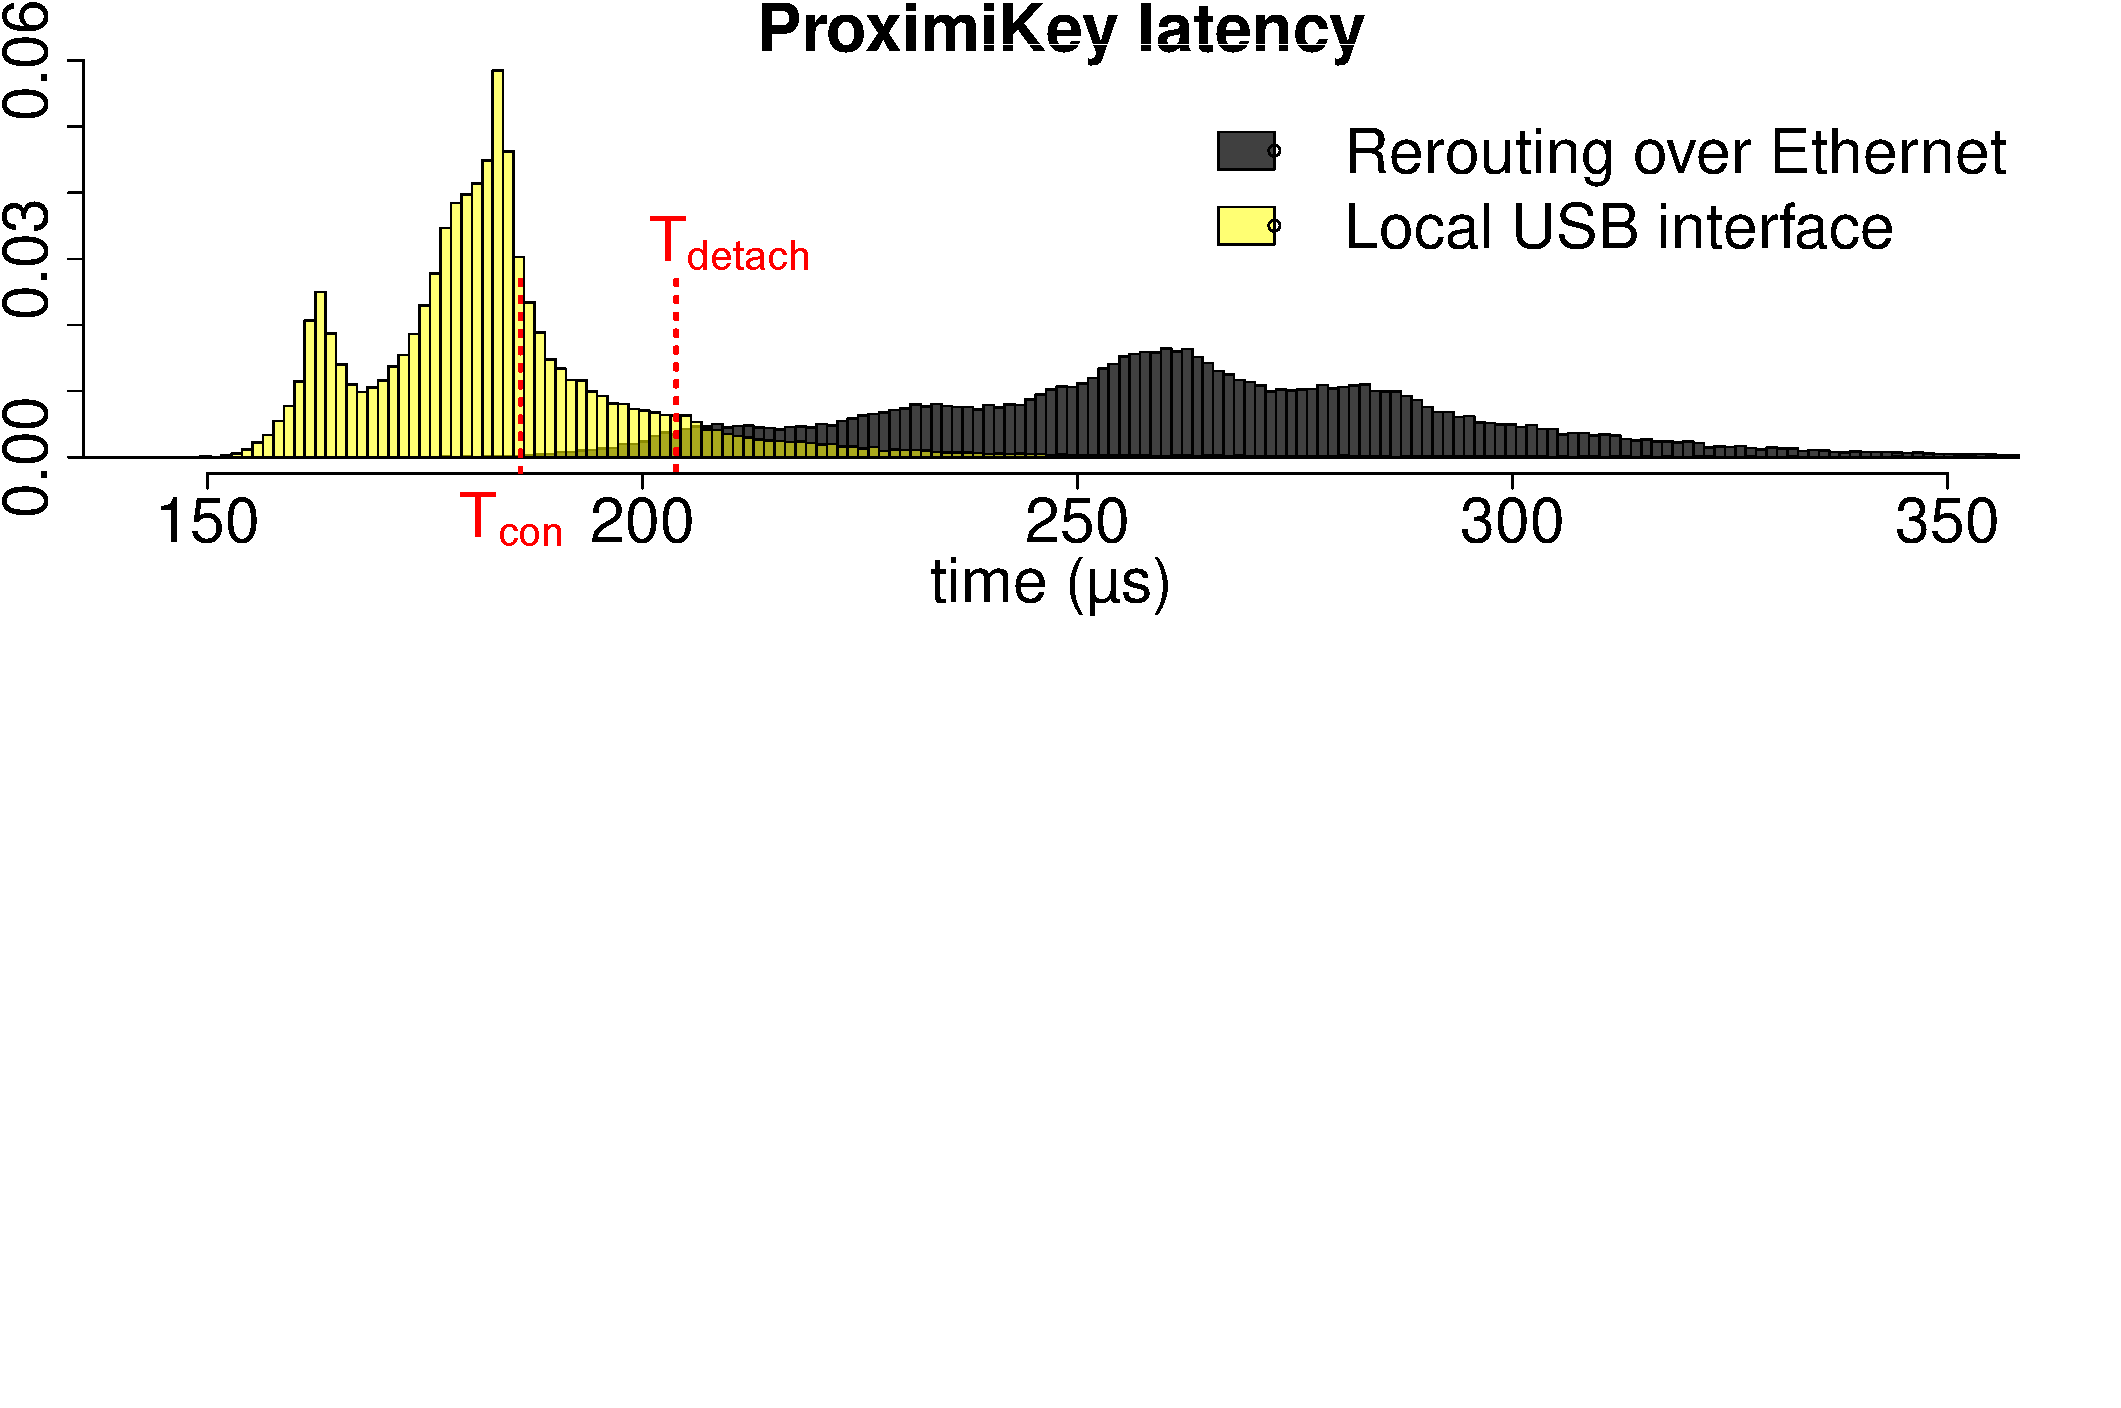
\includegraphics[trim={0 13.4cm 0 0},
    clip,width=\linewidth]{histo.pdf} 
    \caption{Latency distributions for legitimate challenge-response rounds and simulated relay attack.}
    \label{graph:histogram}
\end{figure}

Figure~\ref{graph:histogram} shows the results from our experiments, where we measured both the legitimate and relayed challenge-response latencies. The vast majority of the benign latencies range from $145$ to $250 \mu s$, while the attack round-trips take from $200$ to $750$ $\mu s$. The average delay of our adversary is only $80 \mu s$. (To put this into perspective, even the highly-optimized network connections between major data centers in the same region exhibit latencies from one millisecond upwards.) 

As can be seen from Figure~\ref{graph:histogram}, these two latency distributions are distinguishable. Our analysis confirms that it is possible to set protocol parameters (number of challenge-response rounds, latency threshold, etc.) such that very fast relay attacks can be detected with high probability and legitimate attestations fail only with negligible probability. The full details of the \proximitee system and our analysis can be found from our recent paper~\cite{proximitee}.

